\subsection{Ultrasonic range sensor}
In order to calculate a GSD, the system needs a way to measure the distance from the camera to the ground. This information can be obtained by using an ultrasonic range sensor. \\

The ultrasonic range sensor utilizes high-frequency sound wave pulses to determine the range from the sensor to the object reflecting the pulse back to the sensor. The sensor outputs the time taken from the sound transmission to the detection of the reflected signal, and is then used to calculate the distance from the sensor to the object.\\

\begin{figure}[h]
  \centering
  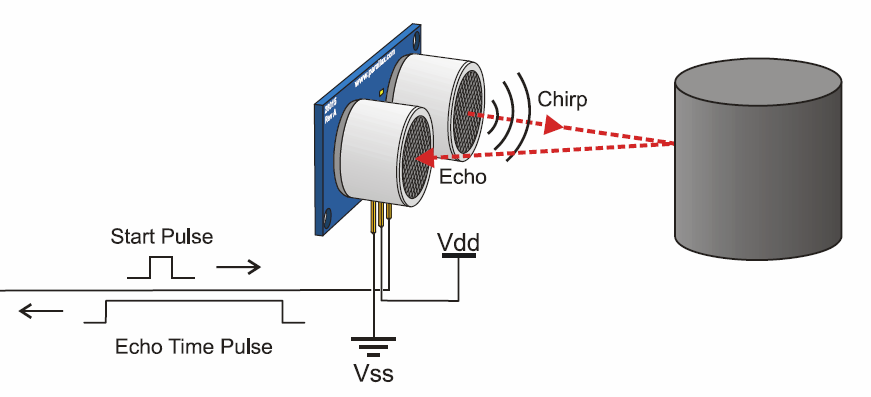
\includegraphics[width=0.7\textwidth]{fig/dsensor}
  \caption{Ultrasonic range sensor. From \cite{maker}}
  \label{fig:dsensor}
\end{figure}

The distance is calculated as follows:
\begin{align}
	speed = \frac{distance}{time}
\end{align}
In dry air at 20 C, the speed of sound is 343 meters per second \cite{sos}. The equation will give the total distance traveled by the sound pulse, so it must be divided by two. Giving:
\begin{align*}
	distance = \frac{speed \times time}{2}\\
    distance = 17150 \times time \quad [cm] 
\end{align*}

\newpage

\subsection{Image Sensor}
The image sensor is one of the most important components in the system. There are several different types of image sensors available, but most of the image sensors we will use consist of an array of small sensors capable of detecting incoming illumination energy and transforming it to digital images.\\

Gonzales explains the process of the digital image sensor as follows: \emph{"The idea is simple: Incoming energy is transformed into a voltage by the combination of input electrical power and sensor material that is responsive to the particular type of energy (wavelength) being detected. The output voltage waveform is the response of the sensors, and a digital quantity is obtained from each sensor by digitizing its response."}\cite{g}\\

That means the response of each sensor in the sensor array of the image sensor is a continuous voltage waveform, and to create digital images from this data the process of sampling and quantization must be applied. Figure \ref{fig:sample} illustrates the the basic idea behind sampling and quantization.
\begin{figure}[h]
  \centering
  \captionsetup{justification=centering}
  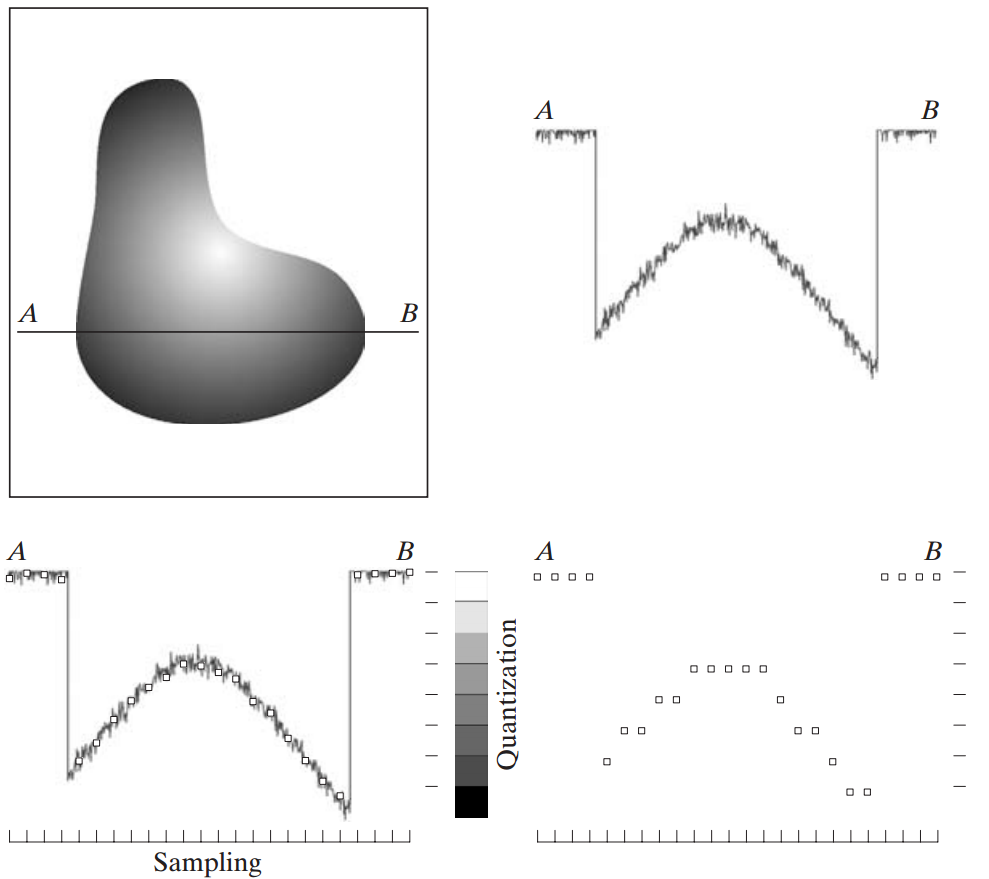
\includegraphics[width=0.7\textwidth]{fig/sample}
  \caption{ Top left: Continuous image\\
  Top right: A scan from A to B in the continuous image\\
  Bottom left: Sampling and quantization\\
  Bottom right: Digital scan line \cite{g}}
  \label{fig:sample}
\end{figure}

Sampling can be described as digitizing the coordinate values of the image, while quantization is the process of digitizing the amplitude values in the image. The amplitude of any given coordinate in the detected image is the intensity value. In terms of our application, it is not vital to understand every detail of how the image sensor works, but a general understanding of the technology is preferred.\\

The image sensor used in this thesis is the IMX219, which is a active pixel sensor CMOS (APS CMOS) image sensor using CMOS technology. APS means that the integrated circuit in the sensor contains an array of pixel sensors, where each pixel contains a photodetector and amplifier.

\begin{figure}[h]
  \centering
  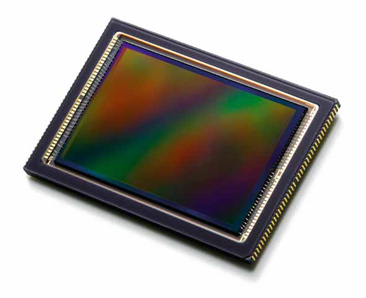
\includegraphics[width=0.4\textwidth]{fig/cmos}
  \caption{APS CMOS Image Sensor}
  \label{fig:cmos}
\end{figure}

Figure \ref{fig:cmos} depicts an APS CMOS image sensor. CMOS is one of the leading technologies for small image sensors often used in mobile phone cameras. CMOS is a technology for designing integrated circuits, and is preferred in image sensors for its small power consumption and small image lag. \\





\newpage
\subsection{Technical hardware requirements}
If a complete image processing algorithm is to be implemented on a mobile computation device, the hardware selected needs to be able to compute and run image processing in a timely manner. Image processing is known to be demanding on hardware, and most advanced implementations such as autonomous cars use high-end dedicated graphic cards \cite{tesla} to be able to run in real time. The algorithm we are implementing does not map in real time, thus the requirements for our hardware performance is reduced. Our hardware should feature enough processing power and storage to be able to run the image processing algorithm as well as storing the image in between operations.\\

These are some of the over-arching hardware requirements:
\begin{itemize}
\item Capable of convolving high resolution images ($>1920\times1080$ pixels)
\item Enough RAM to store images during operations
\item Dedicated graphics chip
\item Powerful enough to be suitable for further project developments into real-time
\end{itemize}

The size of the image output is maximum $3280 \times 2464 $, which makes approximately 8.08M pixels. Since the bit depth of the sensor is 10-bit, I can calculate the file size of the image:

\begin{align*}
3280\times 2464 \quad[pixels] \times 10[bit] = 80819200\quad[bit] = 10102400\quad[bytes]\\
10102400\quad[bytes] \div1048576 = 9,63\quad[Megabytes]
\end{align*}

I assume the image file size is at a maximum $10$ Megabytes for calculation purposes. This means that the hardware needs to provide sufficient RAM to store images of several Megabytes. The GPU should also be able to do operations on pictures of this size, which means a dedicated graphics chip could be beneficial to the system.

%Litt mer

















